\section{Introdução} 
\subsection{Definição justificada dos objetivos e da sua relevância}
A palavra “computador” é usada desde o século XVII, tendo a sua primeira referência escrita datada de 1613. No entanto, por muito tempo “computador” não tinha o mesmo significado que leva hoje, sendo utilizada, até a década de 1940, como nome da profissão de alguém que calcula, segundo o dicionário Michaelis: “Aquele ou aquilo que calcula baseado em valores digitais; calculador, calculista”. \cite{4}

Tendo em vista o antigo significado da palavra “computador”, pode-se questionar sobre como passamos a utilizar uma palavra usada para se referir a pessoas, para maquinas. A fim de responder essa pergunta, recuperaremos a origem dos computadores. Pode parecer um questionamento simples, porém muitas pessoas não sabem a verdadeira resposta. Computadores existem há mais tempo que o transistor – dispositivo semicondutor usado para amplificar ou alternar sinais eletrônicos e eletricidade – na forma mecânica e teórica. A definição de ``computador'' foi elaborada por Alan Turing (Reino Unido, 1912-1954), um matemático, lógico, criptógrafo e herói de guerra que se preocupava exatamente com a questão relacionada ao que era computável e o que não era. Ele foi elaborou a definição de computador, descrevendo a Maquina de Turing, em um trabalho publicado em 1937. A origem dos computadores e celulares que você, leitor, pode estar usando para ler o presente trabalho é fruto do resultado deste trabalho.

A Maquina de Turing, considerada o modelo mais poderoso de computador, é similar a um automato finito\footnote{Um sub-tópico da Ciência da computação teórica, também chamado máquina de estados finita determinística — é uma máquina de estados finita que aceita ou rejeita cadeias de símbolos gerando um único ramo de computação para cada cadeia de entrada.}, porém com uma mémoria ilimitada e irrestrita, constituindo um modelo mais exato de um computador de forma geral. Esta é composta por três principais componentes: fita infinita; processador; máquina de estado finito. 


\vspace{1cm}
\begin{figure}[H] \centering 
  \makebox[\textwidth][c]{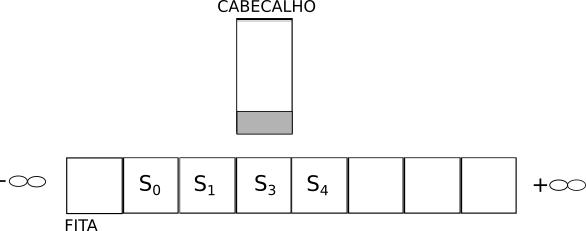
\includegraphics[width=0.8\textwidth]{turing_machine}}
  \caption{\label{fig:1} Desenho esquemático Maquina de Turing} 
\end{figure}

A fita infinita é dividida em células, cada uma contendo um simbolo de um alfabeto finito. O processador é responsável por se deslocar para a direita ou para a esquerda e efetuar a leitura ou escrita em uma célula. Assim, o Prof. Dr. Fabio Gagliardi Cozman\cite{7}, ilustra seu funcionamento da seguinte forma:
\begin{enumerate}
  \item Inicialmente a fita contém somente a cadeia de entrada, disposta no “meio”\footnote{Meio é algo abstrato nesse sentido pois não existe meio de um valor infinito} da fita , com o processador posicionado no início da cadeia (o resto está em branco);
  \item Para armazenar algo, a máquina escreve na fita;
  \item O processador pode ser movido livremente para a esquerda ou direita, afim de ler ou escrever valores em qualquer célula;
  \item As saídas ``aceita'' e ``rejeita'' são obtidas ao entrar nos estados de aceitação e rejeição;
  \item Se não entrar em um estado de aceitação ou rejeição, continuará sua computação para sempre, em  "loop infinito".
\end{enumerate}

O primeiro computador digital eletrônico de grande escala, foi criado em fevereiro de 1946 por cientistas norte-americanos, John Presper Eckert e John W. Mauchly, da Electronic Control Company. No final de sua operação em 1956, o ENIAC (Electrical Numerical Integrator and Calculator), continha 20.000 tubos de vácuo, 7.200 diodos de cristal, 1.500 relés, 70.000 resistores, 10.000 capacitores e aproximadamente 5.000.000 juntas soldadas à mão. Ele pesava mais de 27 toneladas, tinha aproximadamente 2,4m * 0,9m * 30m de tamanho, ocupava 167 m2 e consumia 150 kW de eletricidade. \cite{2}

A partir do ENIAC, as possibilidades tectológicas tomaram uma nova proporção. Em 1969, apenas 13 anos após o desligamento do primeiro computador digital eletrônico, o computador de bordo da Apollo 11 – missão que levou o homem  à Lua – tinha 32.768 bits\footnote{Para uma explicação elaborada sobre bits refira-se ao capítulo \ref{bits} pagina \pageref{bits}} de RAM, o suficiente para armazenar apenas um texto não formatado, com cerca de 2.000 palavras. O que contrasta com o Iphone XS com 4gb de RAM, que em 2018, tinha cerca de 1 milhão de vezes mais de memória que o Apollo Guinche Computer. \cite{5}

\vspace{1cm}
\begin{figure}[H] \centering 
  \makebox[\textwidth][c]{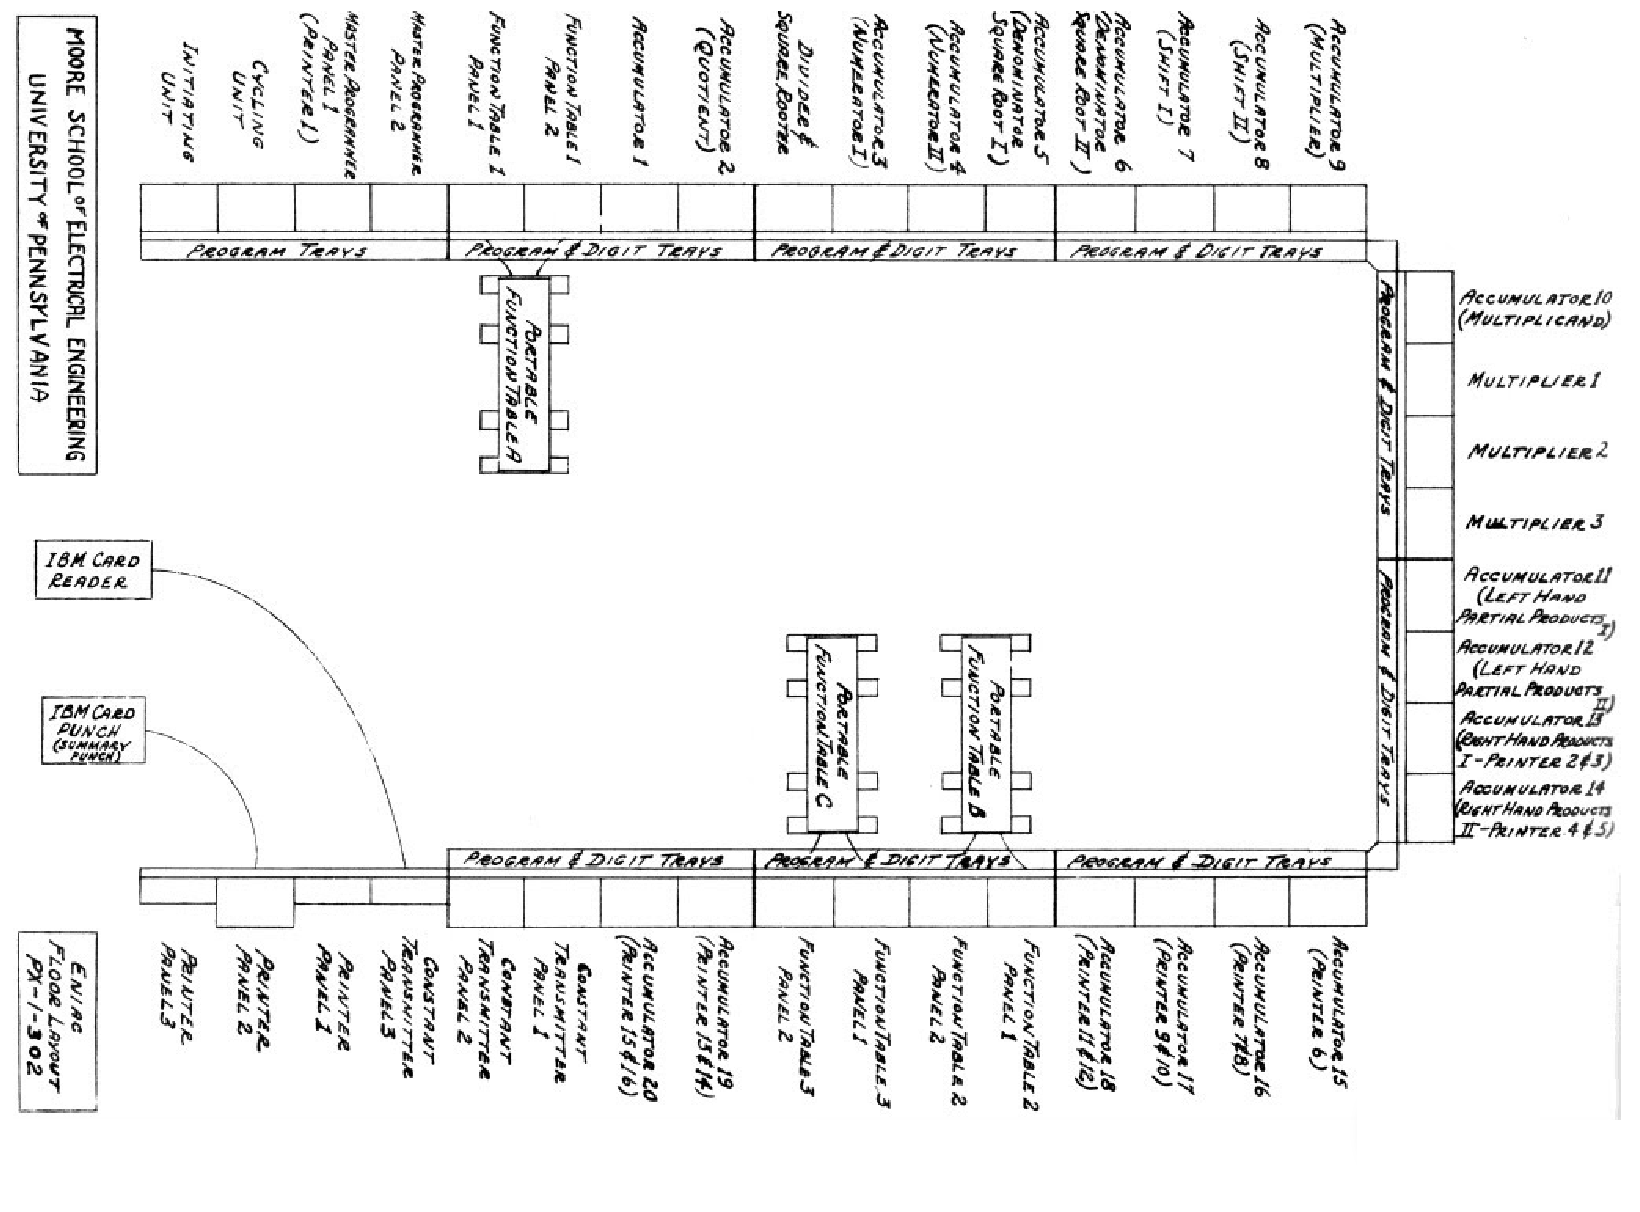
\includegraphics[width=0.8\textwidth]{ENIAC_floor_layout}}
  \caption{\label{fig:2} Desenho esquemático do ENIAC/US Center for Military History –
  Adele Goldstine} 
\end{figure}

% (falar da Spacex e falcon9 e CRS-12 Dragon 2020)

Durante o século XX, além do aumento do poder computacional dos dispositivos, outro fator impactante foi a refatoração de seus tamanhos. Assim, com tecnologias wearables\footnote{A tecnologia em questão não somente pode ser usada como uma peça de roupa ou um acessório, como também tem que possuir características que a conectem a outros aparelhos ou à internet.}, os computadores se tornam ativamente presentes no cotidiano.

Levando em consideração o rápido avanço e desenvolvimento computacional, mencionados anteriormente, entende-se que os computadores agregam à sociedade, seja facilitando a comunicação e o compartilhamento de conhecimentos, como em outros aspectos. No entanto, a agilidade pela qual se deu tais \textbf{transformações da tecnologia da computação}, também gera grandes expectativas e incertezas sobre o que ainda está por vir, tanto nas questões de mudanças tecnológicas quanto nos impactos na sociedade.

Tendo em vista a incerteza que acompanha o futuro da computação e de seus próximos avanços, a presente pesquisa se propôs a estudar os conceitos da física clássica e da física quântica aplicados à computação, além do estudo dos princípios da criptografia\footnote{Criptografia é um sistema de algoritmos matemáticos que codificam dados para que só o destinatário possa ler.}. Com base nesses conceitos será prototipado um computador clássico de 8 bits em hardware usando apenas portas lógicas simples, de forma a possibilitar um ilustração clara do funcionamento. Junto a isso será desenvolvida uma aplicação web que ilustre o funcionamento de um processador quântico. Ao final, conceitos de criptografia serão utilizados para exemplificar possíveis mudanças sociais que os próximos avanços tecnológicos podem gerar.

\subsection{Metodologia a ser empregada}
Para a realização da pesquisa de iniciação científica, é indispensável o uso de pesquisa bibliográfica, afim de recuperar e se aprofundar no conhecimento cientifico. Segundo Telma Cristiane Sasso de Lima, o conhecimento da realidade não é apenas a simples transposição dessa realidade para o pensamento, mas sim a reflexão crítica, que se dá a partir de um conhecimento acumulado que irá gerar uma síntese, o concreto pensado \cite{1}. E também a utilização do processo científico para a elaboração e efetivação do projeto em si. Ambas metodologias citadas acima, são cruciais para o desenvolvimento do relatório final na área de pesquisa em computação, já que em grande parte dos estudos, a utilização do processo científico é frequentemente utilizada para um maior entendimento da obra e a construção do projeto se tornar mais facilmente executável.

Assim, para o desenvolvimento da entrega do protótipo – computador de 8-bits – e para o simulador do computador quântico web, a principal metodologia utilizada será O Project Based Learnig (PBL). De acordo com  David Van Andel, o PBL envolve os alunos em um processo rigoroso de investigação, onde eles fazem perguntas, encontram recursos e aplicam informações para resolver problemas do mundo real \cite{3}. Assim, entende-se que esta é a melhor metodologia para desenvolver um protótipo físico de um computador e programar um site.

\newpage